\chapter{開発準備}

\section{開発に利用したツールとその経緯}%例:レビュー内容
%必要ならここに大見出しの内容
%必要なら下のsubsectionを用いて小見出しをつかう
\subsection{Monaca}%:発表技法について
iOSとAndroidの両方のプラットフォームでアプリケーションを使いたいという町会の要望を叶えるために, HTML5ハイブリッドアプリを開発することとした. iOSとAndroidには, 「WebView」と呼ばれるブラウザの機能を持つコンポーネントが組み込まれている\cite{book_about_monaca}. HTML5ハイブリッドアプリとは, 「WebView」にHTMLとCSS, JavaScriptを用いて開発するアプリケーションである\cite{book_about_monaca}. また, HTML5ハイブリッドアプリの開発ツールのなかからMonacaを選択した. MonacaはCordovaというオープンソースのフレームワークを利用している\cite{book_about_monaca}. また, MonacaにはMonacaクラウドIDE, Monaca Localkit, Monaca CLIの3種類の開発環境が存在する\cite{book_about_monaca}. MonacaクラウドIDEは, インターネットクラウド上で開発するため個人の開発環境に依存しない\cite{book_about_monaca}. Monaca Localkitは, MonacaクラウドIDEとは異なり, 各メンバごとにローカルでの開発を可能とする\cite{book_about_monaca}. Monaca CLIは, MonacaクラウドIDEが提供するサービスを, コマンドライン形式で利用することを可能にする\cite{book_about_monaca}. いずれの開発環境においても, Monacaデバッカーを用いて, デバックを行う(図\ref{fig:image_monaca}).

\begin{figure}[h]
  \begin{center}
  %\begin{flushleft}
    \begin{tabular}{c}

      % 1
      \begin{minipage}{0.7\hsize}
        \begin{center}
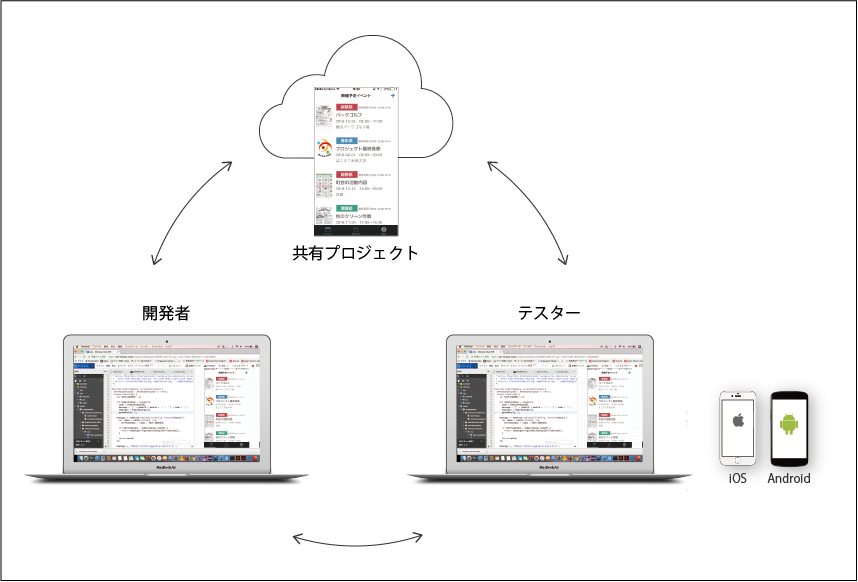
\includegraphics[width=10cm]{monaca_overview.png}
          \hspace{1cm} %(a)観光スポットの紹介
        \end{center}
      \end{minipage}

    \end{tabular}
    \caption{Monacaでの開発イメージ\cite{monaca_debugger}}
    \label{fig:image_monaca}
  \end{center}
  %\end{flushleft}
\end{figure}

\subsection{ニフティクラウド mobile backend}%:発表技法について
本アプリケーションの各情報を保存する場所として, mBaaSの1つであるニフティクラウド mobile backend(以下, NCMBとする)を使用した. 使用した理由として, 以前このサービスを利用したことがあること, 他のmBaaSと比べて無料で利用可能な機能多いことが挙げられる. mBasSとは, サーバーの開発, 運用を必要とせずユーザから直接見えない部分の機能をアプリケーションに実装することを可能にするサービスである\cite{about_mbaas}. NCMBは, プッシュ通知, 会員管理と認証, SNS連携などの機能\cite{price_mbaas}を提供しているサービスである(図\ref{fig:image_mbaas}).

\begin{figure}[htbp]
%\begin{flushleft}
  \begin{center}
    \begin{tabular}{c}

      % 1
      \begin{minipage}{0.7\hsize}
        \begin{center}
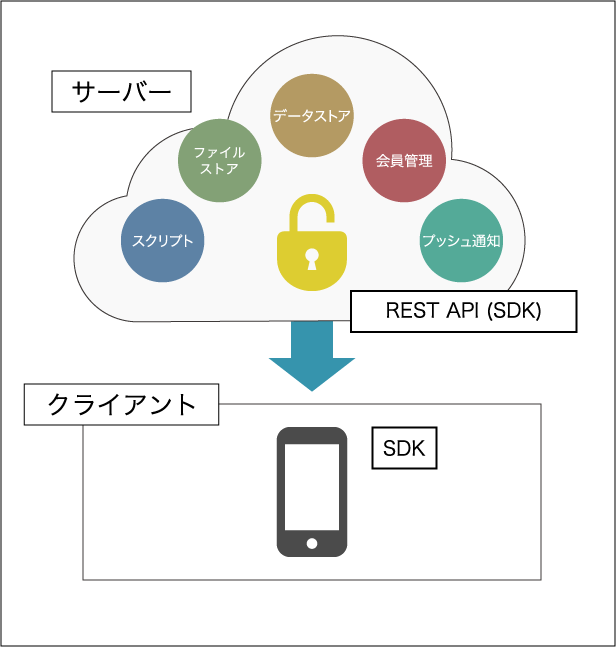
\includegraphics[width=10cm]{ncmb_overview.png}
          \hspace{1cm} %(a)観光スポットの紹介
        \end{center}
      \end{minipage}

    \end{tabular}
    \caption{ニフティクラウド mobile backendのサービス内容\cite{intro_mbaas}}
    \label{fig:image_mbaas}
  \end{center}
  %\end{flushleft}
\end{figure}


\subsection{Git/GitHub}%:発表技法について
ソースコードのバージョン管理ツールとして, Git/GitHubを使用した. Gitはファイルの変更履歴をリポジトリと呼ばれる場所に保存する. そのため, 一度編集したファイルを過去の状態に復元することや, 編集箇所を表示することが可能となる\cite{book_about_github}. リポジトリの種類は, メンバのローカルPC内に存在するローカルリポジトリと, インターネット上に存在するリモートリポジトリの2種類である\cite{monkey_git}. リモートリポジトリでは, 各メンバのファイルの変更履歴を保存し, 共有する事が可能である. GitHubは, リモートリポジトリを提供するサービスの1つである. これにより, 複数のメンバで同時に開発を進めることが可能となった.

\subsection{Slack}%:発表技法について
チーム内のコミュニケーションツールとして, Slackというチャットツールを使用した. Slackには数多くの特徴や機能が備わっているが, 本プロジェクトでは以下の2個の機能を主に使用した. 1つ目は, 一つのteamに対して複数のチャンネルを作成することができる機能である. Slackはまず最初にteamというものを作成する. これは, teamの名前は"2016プロジェクト03"など, 団体名やプロジェクト名で名付ける. その後, 議題ごとに"\#report"や"\#design"などとチャンネルを作成することが出来る. これらの機能のお陰で, 1つの話題について見逃すこと無く, 集中して話し合うことができた. また, ファイルやリンクの共有についても同様に, チャンネルごとに分けて行うことができた. 2つ目は, GitHubなどの他のサービスと連携することができる機能である. 連携先のGitHubに何らかの変更が生じた時に, 指定したチャンネルに通知が来るように設定した. この機能のお陰でアプリケーションや報告書に変更があった場合に, グループメンバ全員が進捗の把握をしやすい環境を整えられた.

\subsection{Redmine}%:発表技法について
タスク管理ツールとして前期は, Redmineというオープンソースソフトウェアを使用した. Redmineでは, 発生したタスクごとにチケットと呼ばれるものを発行する. その後, タスクの進捗に合わせて各チケットを新規, フィードバック, 進行中(着手), 進行中, 進行中(終了間際), 作業終了, レビュー中, 完了, 却下の9段階に分ける. また, チケットには担当者を指定し, チケットが更新される度に通知が来るようにウォッチャーと呼ばれるものに各メンバを設定する. これにより, 各メンバのタスクの進捗状況を把握することが可能となった.しかし, 機能の多さからなる操作の複雑さや, チケットの変更を受動的に知ることができないといった理由から, 後期は使用を見送った。

\subsection{Trello}%:発表技法について
タスク管理ツールとして, 後期からTrelloを使用した. Trelloでは, タスクを「カード」として登録し, 「ボード」と呼ばれる場所で管理する\cite{Trello}. その後, todoやdoneなど好きな名前で「リスト」を作成し, 進捗状況に合わせて「カード」を移動することで, 進捗を管理する\cite{Trello}(図\ref{fig:image_trello}). また, ボードは個人で使うこともチームで共有することもできる\cite{Trello}. 完了した「カード」はアーカイブする. 私たちは, 「カード」が移動されると, チームで使用している連絡ツールに通知が来るように設定をした. これにより, Redmineよりも迅速に進捗を把握することができた. さらに, 通知が来た後そのまま連絡ツールで, 話し合いをすることもできた.
%参照先 https://seleck.cc/610
\begin{figure}[htbp]
%\begin{flushleft}
  \begin{center}
    \begin{tabular}{c}

      % 1
      \begin{minipage}{1\hsize}
        \begin{center}
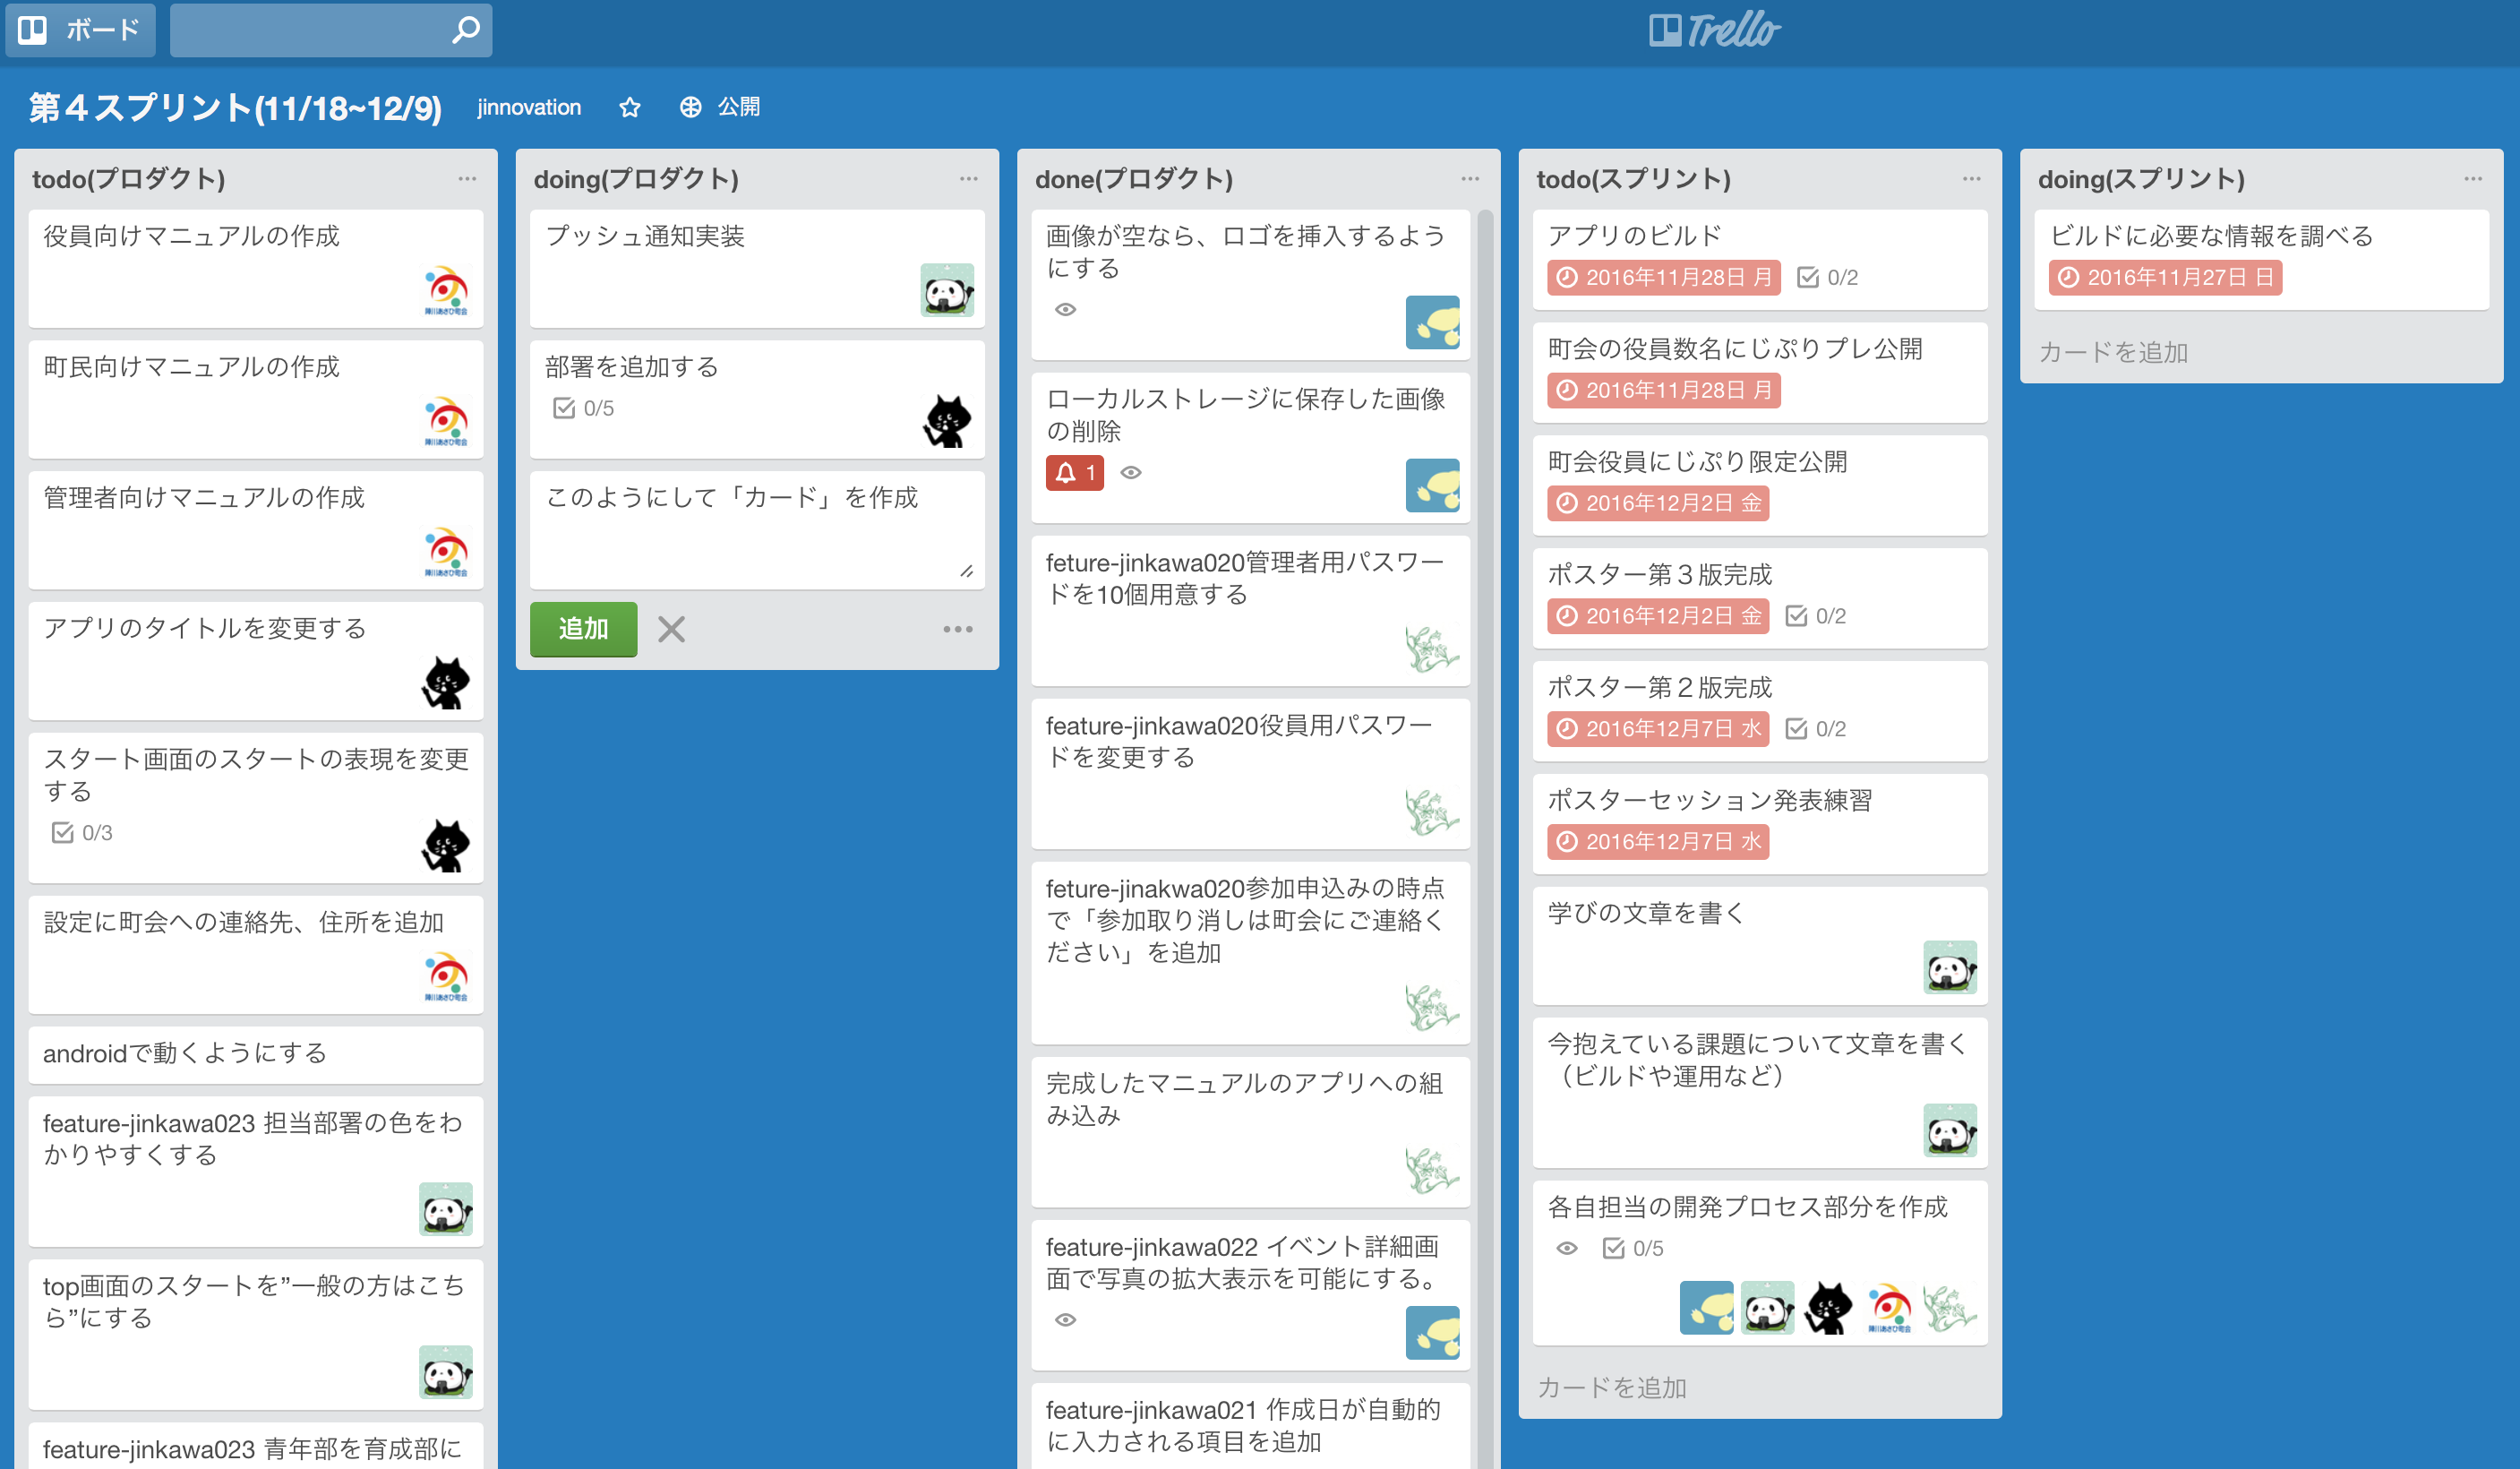
\includegraphics[width=14cm]{about_trello.png}
          \hspace{1cm} %(a)観光スポットの紹介
        \end{center}
      \end{minipage}

    \end{tabular}
    \caption{実際に使用したTrelloの「ボード」}
    \label{fig:image_trello}
  \end{center}
  %\end{flushleft}
\end{figure}

\subsection{Adobe Illustrator}%:発表技法について
ポスター作成と開発するアプリケーションのイメージ図の作成にAdobe Illustratorを使用した. Adobe Illustratorはイラストやポスターなどデザインを描画するソフトウェアの1つである.

\bunseki{船木綾香}

\section{環境構築}%例:レビュー内容
Monacaの3種類の開発環境の中から, オフラインで作業する可能性があることと普段使い慣れているエディターで開発することが望ましいため, Monaca CLIを選択した. Monacaの公式Webサイト\cite{tutorial_monaca_CLI}を見ながら, Monacaアカウントの作成, Monaca CLIのインストール, コマンドラインからMonacaへのログイン, 新規プロジェクト作成の順で環境構築を行った. GitHubについては, リモートリポジトリに機能やバグの修正ごとにブランチを作成し, そこにプッシュするようにした. また, リモートリポジトリにdevelopブランチを作成した. このdevelopブランチは, 各ブランチの内容をマージするためのブランチである. このdevelopブランチを作成した理由は, 単体テストを終えた各ブランチの内容をmasterブランチにマージする前に, developにマージすることで, 結合テストを行うためである. また, masterの内容を常に安定した状態に保つという役割も担っている. Slackについては, 教員が用意したteamにメンバ全員が参加し, 町内会グループ専用の"\#jinkawa"チャンネルを用意した. 前期に使用したRedmineは, 担当教員よりすでに構築済みのものを提供していただいた. 原則ウォッチャー\cite{Redmine}は, メンバ全員を登録することとした. 後期に使用したTrelloは, 各自アカウントを作った後, ボードを共有することでタスク管理を行った. また, チームで利用しているチャンネルと連携させることで, チャンネル内でタスクの状況を把握できるようにした.

\bunseki{横山新}
